\chapter{ErsteErfahrung} \label{cha:ErsteErfahrung}

In diesem Kapitel werden die erste Erfahrung beschrieben. Zuerst läuft die Vorstellung des DaVid-Systems. Die Systemmodell und Arbeitsprinzip des Systems werden in anschließenden Abschnitt erläutert. Schließlich folgt die mögliche Anwendungsgebiete des Systems.

Nicht vergessen, dass Überschriften nicht aufeinander folgen dürfen\ldots

\begin{otherlanguage}{english}
\section{TexLipse spell checking}
%
To enable spell checking in TeXLipse, download the respective dictionaries from 
\url{https://sourceforge.net/projects/texlipse/files/dictionaries/}.

Save the dictionaries at a local location and enter the path in \texttt{Window->Preferences->Tex\-lipse->Spell Checker} (see Fig. \ref{fig:dict_path}).
%
\begin{figure}[htb]
	\centering
	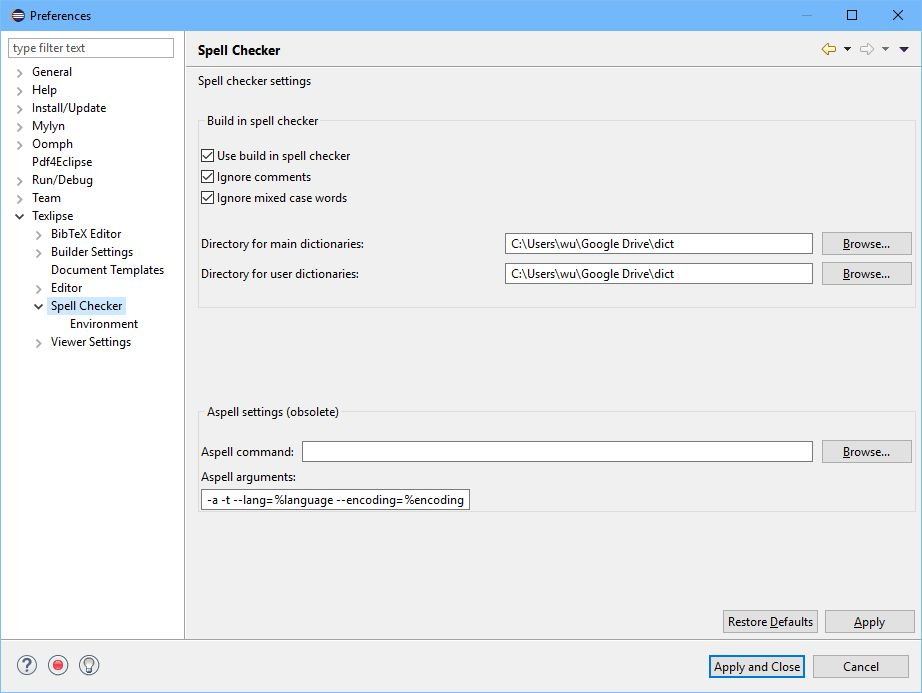
\includegraphics[scale=0.40]{images/Spell_Checker_preferences.jpg}
	\captionbelow{TeXLipse Spell Checker preferences}
	\label{fig:dict_path}
\end{figure}

To synchronize the user dictionaries between multiple machines, it might be useful to save the dictionaries in your google drive or drop box.

\section{Enable tikzexternalize for PdfLatex}

Go to \texttt{Window->Preferences->Texlipse->Builder Settings} and add 
%
\begin{verbatim}
--shell-escape
\end{verbatim}
%
to the command arguments (see Fig. \ref{fig:builder_settings}).
%
\begin{figure}[htb]
	\centering
	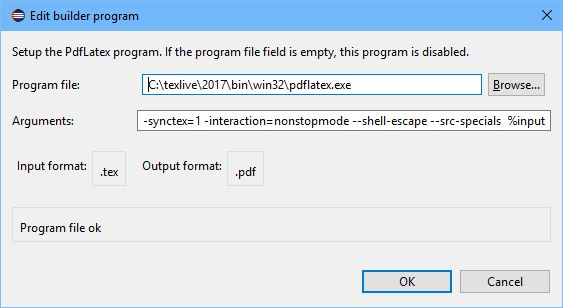
\includegraphics[scale=0.40]{images/PdfLatex_settings.jpg}
	\captionbelow{PdfLatex Builder Settings}
	\label{fig:builder_settings}
\end{figure}

\section{Forward search with TeXlipse and Sumatra PDF}

Download and install SumatraPDF: \url{https://www.sumatrapdfreader.org/}.

Then edit the viewer settings for SumatraPDF in \texttt{Window->Preferences->Texlipse->Viewer Settings}.

Change the viewer arguments to
%
\begin{verbatim}
-reuse-instance %fullfile -forward-search %texfile %line
\end{verbatim}
%
and leave all DDE message field empty.
Change the inverse search support to "`Viewer runs external command"' and enable "`Viewer supports forward search"'.

Figure \ref{fig:viewer_settings} displays the dialog window.
%
\begin{figure}[htb]
	\centering
	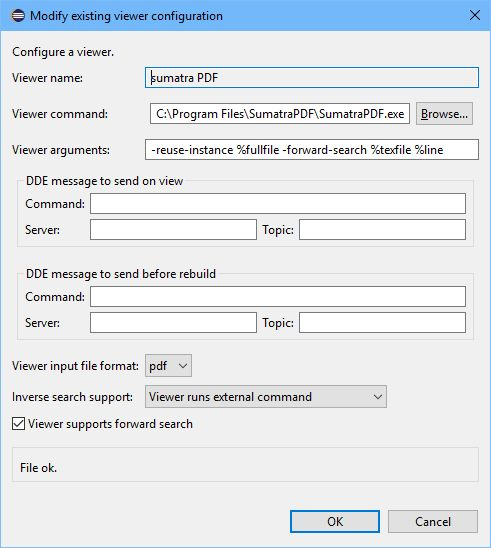
\includegraphics[scale=0.40]{images/Viewer_settings.jpg}
	\captionbelow{TeXLipse Viewer Settings}
	\label{fig:viewer_settings}
\end{figure}

In SumatraPDF configure the inverse search command via the \texttt{Settings->Options} menu (see Fig. \ref{fig:sumatrapdf_options}).
%
\begin{figure}[htb]
	\centering
	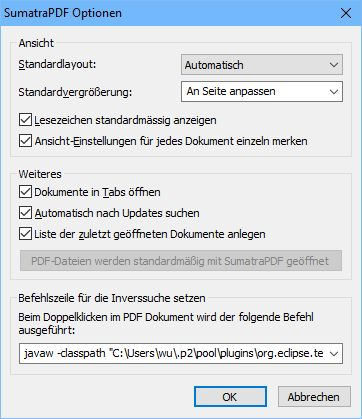
\includegraphics[scale=0.40]{images/SumatraPDF_optionen.jpg}
	\captionbelow{SumatraPDF Options}
	\label{fig:sumatrapdf_options}
\end{figure}

If you have install TeXlipse~1.5.0, the inverse search command will look like this:

\begin{lstlisting}[breaklines=true, basicstyle=\ttfamily, columns=flexible]
javaw -classpath "C:\Users\wu\.p2\pool\plugins\net.sourceforge.texlipse_1.5.0\texlipse.jar" net.sourceforge.texlipse.viewer.util.FileLocationClient -p 55000 -f "%f" -l %l
\end{lstlisting}

Let the path point to your eclipse share pool. Or if you do not have a shared pool, choose the plugins directory of your eclipse installation.

For TeXLipse~2.0.X the FileLocationClient is relocated to org.eclipse.texlipse making the inverse search command look like the following.
\begin{lstlisting}[breaklines=true, basicstyle=\ttfamily, columns=flexible]
javaw -classpath "C:\Users\wu\.p2\pool\plugins\org.eclipse.texlipse_2.0.1.201801202105\texlipse.jar" org.eclipse.texlipse.viewer.util.FileLocationClient -p 55000 -f "%f" -l %l
\end{lstlisting}

\end{otherlanguage}